% Chapter Template

\chapter{Design} % Main chapter title

\label{Chapter4} % Change X to a consecutive number; for referencing this chapter elsewhere, use \ref{ChapterX}

 
%----------------------------------------------------------------------------------------
%	SECTION 1
%----------------------------------------------------------------------------------------

\section{Requirements}

Requirements are distinguished into the two categories, functional, and non-functional. Each category has requirements specified for the user, and for a developer. A user is a person that use or communicate with the component in the form of actions like searching or filtering. Requirements are defined based on the assignment as well as based on the functionalities of the current solutions.

%----------------------------------------------------------------------------------------
%	SUBSECTION 1.1
%----------------------------------------------------------------------------------------

\subsection{Functional}

Functional requirements related to the user are following:
\begin{enumerate}
    \item Component must support multiple options providers
    \item Dropdown with results will be displayed on focus
    \item Each option should show its state (additional info such as - comment, providers, or its state)
    \item User must be able to filter among these options
    \item Selection and multi-selection must be provided
    \item The component must provide a way to create new options
    \item The component should accept and visualize tree-structured data.
\end{enumerate}
Other functional requirements for developers
\begin{enumerate}[resume]
    \item The component must be able to work with linked data sources
    \item The component should support multiple input formats – JSON (because of the easy interpretation on the client side) and XML (because of the wide marketplace) 
\end{enumerate}

%----------------------------------------------------------------------------------------
%	SUBSECTION 1.2
%----------------------------------------------------------------------------------------

\subsection{Non-Functional}

Non-functional requirements
\begin{enumerate}
    \item Operations like search and render must be scalable without negative impact on the user experience
    \item Processing data, filtering and rendering should be real-time (not take longer than acceptable)
\end{enumerate}
Other non-functional requirements for developers
\begin{enumerate}[resume]
    \item Component must be easily integrable with React applications
    \item Component must be flexible – custom styling, own filter method and render method
\end{enumerate}

%----------------------------------------------------------------------------------------
%	SECTION 2
%----------------------------------------------------------------------------------------

\section{Use-cases}
 
Based on the requirements, I identified the following use-cases. There are two actors, a developer and a user of the component. The focus of the use cases for the user is mainly on the interaction between user and data displayed by the component in the form of options. On the other hand for the developer use-cases are focused on the needs to integrate the component into their applications.
 
 \begin{figure}[th]
    \centering
    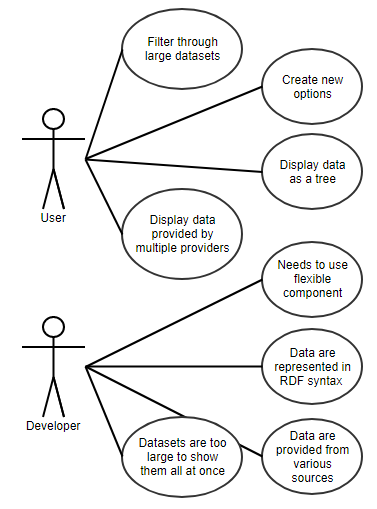
\includegraphics[width=.7\textwidth]{use-case-diagram}
    \decoRule
    \caption[Use Case diagram]{Use Case diagram}
    \label{fig:use-case-diagram}
 \end{figure}

%----------------------------------------------------------------------------------------
%	SECTION 3
%----------------------------------------------------------------------------------------

\section{Providers APIs research}

Firstly, lets quickly introduce what Application  Programming Interface ( API ) is. API stands for Application Programming Interface. It is a program layer that is responsible for interacting with users, giving them responses based on their request. We will be focusing only on Web API. The simplest way to describe Web API is that Web API is set of dedicated web URLs, somewhere on the internet that return some response (usually in text format) to the requestor. There are several types of Web APIs. From historical SOAP (Simple Object Access Protocol) \parencite{soap} and SOA to more modern REST (Representational State Transfer) \parencite{rest}. Because nowadays usage of the REST API is highest, let's focus only on this one type. I will be using Spotify API \parencite{spotify_api} as an example, because of their excellent documentation and variety of their endpoints. All Web APIs have three parts. As you can see below, first is their root address, in this case, it is https://api.spotify.com then following a version, but this is an optional part. Next is an endpoint /artists/{id}/albums; notice a {id} parameter in the URL, this is one way how to send some data to the API. Last part is query parameter. Query parameters are at the end of the URL behind question mark and contain key=value pairs connected with an ampersand. Usually, all query parameters are optional because they have a default value specified on the API side.

\vskip 0.1in

\noindent \colorbox{ltGray}{\parbox{\textwidth}{\textcolor{black!90}{\nolinkurl{https://api.spotify.com/v1/artists/1vCWHaC5f2uS3yhpwWbIA6/albums?market=ES&album_type=single&limit=2}}}}

\vskip 0.2in

Each HTTP \parencite{http} request must also have a header part, where are specified some other information. E.g. Accepted-language or encoding, but most important are Referer and Host.

\begin{figure}[th]
    \centering
    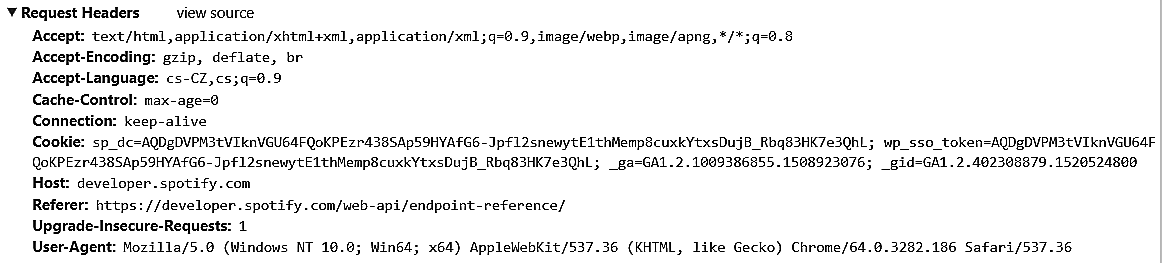
\includegraphics[width=\textwidth]{request_header}
    \decoRule
    \caption[Request header]{Example of request header}
    \label{fig:request_header}
 \end{figure}

Last part of each request is body part. This is the second way how you can send or get some data. But the data format must be in a format that is supported by the server side. The most commonly-used data format is JSON or XML. Often the service supports multiple formats, and the client can request one or the other by including 'json' or 'xml' in the header field 'Accept'.

The functionality of the Web API is much more complicated. The main problem is the complexity; each API can have different behavior based on what data format provides. As I mentioned earlier, most common data formats are JSON or XML. These are both text file formats, but you can also get images, web pages, music file and much more.

There are some examples of the Web APIs that returns different data types.

\begin{itemize}

\item returning json file: https://api.spotify.com/v1/artists/6sFIWsNpZYqfjUpaC gueju 
\item returning web page: https://open.spotify.com/artist/0OdUWJ0sBjDrqHygG UXeCF
\item returning image: https://u.scdn.co/images/pl/default/438f9b65ac4eb48681
351593142daeb070986293
\item returning music file: https://p.scdn.co/mp3-preview/3eb16018c2a700240e9d
fb8817b6f2d041f15eb1?cid=774b29d4f13844c495f206cafdad9c86
\end{itemize}


Some APIs supports filtering in the server side so you can create a requests to get a specific data you want. For example, this API returns 10 artists whose name contains 'tania'
\begin{itemize}
\item \nolinkurl{https://api.spotify.com/v1/search?q=tania%20bowra&type=artist&limit=10}
\end{itemize}

Most of the time API returns only simplified data object, and to get the full information you must request it with for that specific ID.
\begin{itemize}
\item \nolinkurl{https://api.spotify.com/v1/artists/1vCWHaC5f2uS3yhpwWbIA6/albums} 
\end{itemize}
This request return an object with an array of simplified album objects. To get the full detail of the album object another request must be made. 
\begin{itemize}
\item \nolinkurl{https://api.spotify.com/v1/albums/43977e0YlJeMXG77uCCSMX}
\end{itemize}
This request returns a full album detail.

\bigskip

In conclusion, there is a lot of different Web API types. You can distinguish them based on their response format (JSON, XML, img, CSV, etc.), type of their response – some supports filtering results on their side, some return an only limited amount of data, while another may return only header information (e.g., IDs), so you must make another request for each ID to get detailed information. 
So in my component, I will provide an interface through which user can define how to handle communication with specific option provider (Web API)


%----------------------------------------------------------------------------------------
%	SECTION 4
%----------------------------------------------------------------------------------------

\section{Component architecture}

Firstly let's have a look at the high-level view. Structure of the Intelligent Tree Data Management component consists of the three main parts or sub-components. The core sub-component is called Virtualized-tree-select and represent the input field with a drop-down menu. The second one is component representing modal form for creating new options. And the last one exposes some settings to the UI so the user can change the behavior of the component. Both Settings and Modal form sub-components, together with the main component communicate with Redux store, where all necessary data are stored. The third sub-component is independent on the Redux store because all necessary data are passed down as props from the parent component. More about each sub-component will be described in next chapter.

\begin{figure}[th]
    \centering
    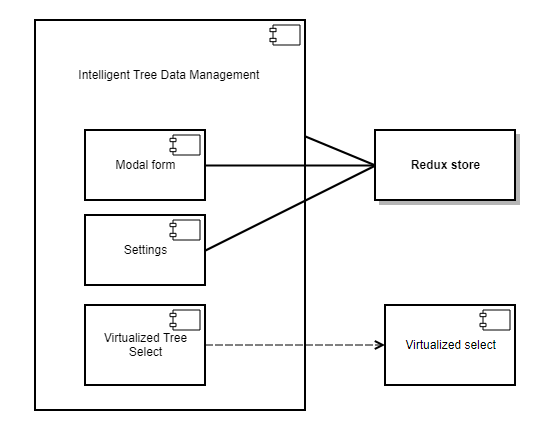
\includegraphics[width=.7\textwidth]{component-diagram}
    \decoRule
    \caption[Architecture]{Component architecture}
    \label{fig:structure}
 \end{figure}

In a low-level point of view, let's look at the UML \parencite{uml} class diagram. As you can see in the image below, main class have three important methods. First method 'onInputChange' check if current input is in history if not, then it call 'getData' for each provider,  and then call 'addNewOptions'. The second method fetches data from providers and returns an array of results. The last method takes the results of the previous call, merge them based on priorities and save it to the already saved options. Other three classes are described in detail in chapter \ref{Chapter5} section 5.2 Component parts. 

The last one is not quite a class, but rather an object of a specific shape. Each option has one or more providers. Provider defines the option characteristics and provides some functions. First function 'response' should return result from the provider. Second one 'toJsonArr' format that response to the array of JSON objects if necessary, and the last one is called only if the label is not a string but array of objects. ( e.g. label: [\{'lang': 'en', 'value': 'This is label'\}, \{'lang':'de', 'value': 'Das ist Label' \}] ). Definition of all properties is in the appendix \ref{AppendixA}.

The association between Provider and Option is 1..N: 1..M because each provider can provide the infinite number of options, but at least it must provide one option. From the other side, it is the same. Each option must have at least one provider. For options that are provided locally the provider called 'local provider' is assigned. 
Next, there is a reflexive association, where each option cant has more than one parent node and N children nodes. Because if you have an option with more than one parent node, then the data cannot be represented as a tree graph.
Last association is between enum class called Type. This class represents the state of the option. Each option can have only one state. However, the state can be contained in N options.

\begin{figure}
    \centering
    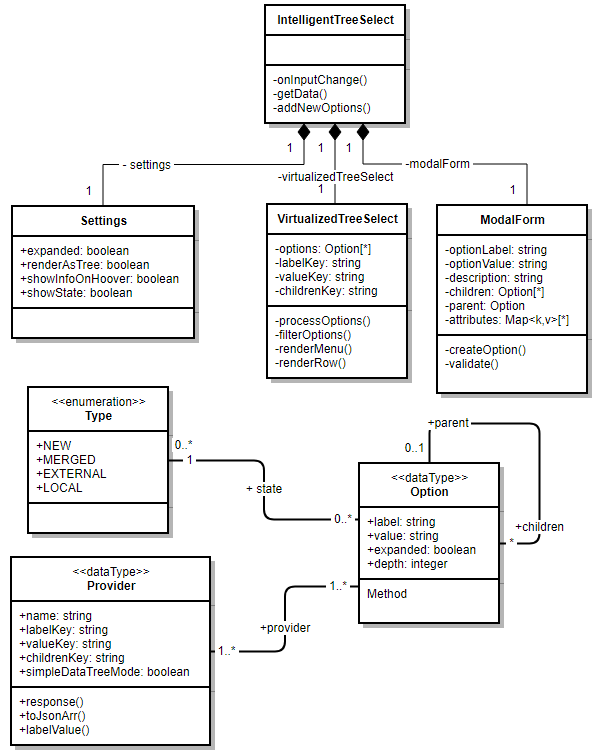
\includegraphics[width=.85\textwidth]{itdm_class_diagram}
    \decoRule
    \caption[Class Diagram]{Component model structure visualized as a class diagram}
    \label{fig:itdm_class_diagram}
 \end{figure}


%----------------------------------------------------------------------------------------
%	SECTION 5
%----------------------------------------------------------------------------------------
\pagebreak

\section{Component life cycle and search cycle}

I will not describe how React handle classes life cycle, because it is not a part of this theses. Also, I will not describe step-by-step of component initialization because it is 
\begin{wrapfigure}{r}{.6\textwidth}
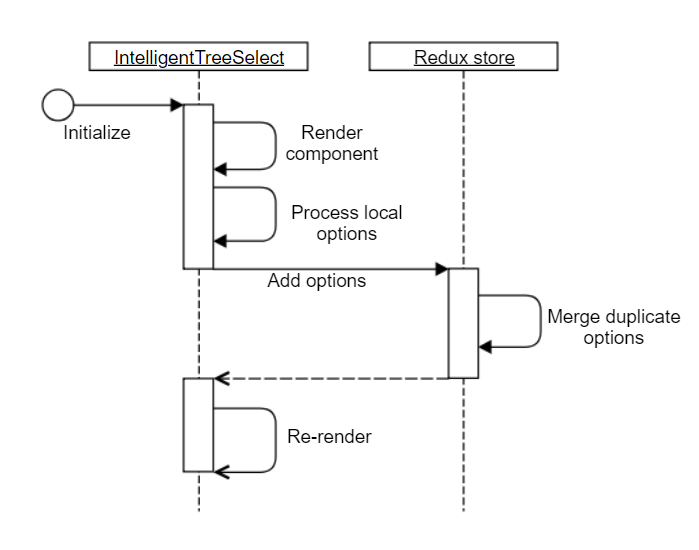
\includegraphics[width=.6\textwidth]{init-sequence-diagram}
    \caption[Initialization]{Component Initialization process}
    \label{fig:init}
\end{wrapfigure}
an out-of-the scope of this thesis. Official React \parencite{react} documentation provides all the necessary information needed. So shortly, as you can see in this image below, the initialization process is divided into three parts. In the first part, the Redux store is created, and all variables (props) are saved. Then the actual HTML elements are rendered and in the last part. If local options are set then they are passed to the virtualized-tree-select sub-component, where they are processed, sorted and the tree graph is created.

\vspace{1cm}

Search cycle is a little bit complicated because some actions are not handled by me, but by the \cite{react-select} and \cite{react-virtualized-select} components. However, I can 
\begin{wrapfigure}{r}{.6\textwidth}
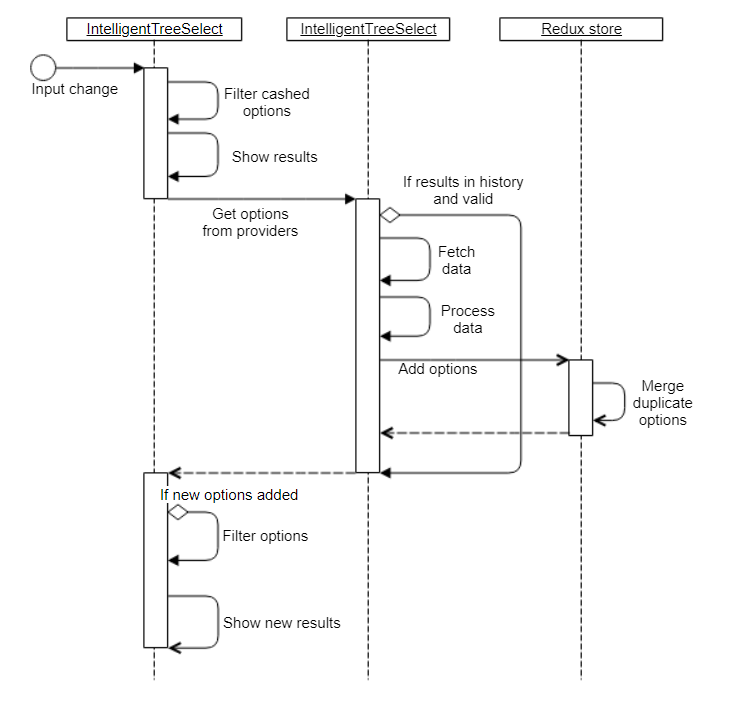
\includegraphics[width=.6\textwidth]{search-sequence-diagram}
    \caption[Search diagram]{Search process}
    \label{fig:search}
\end{wrapfigure}
describe this process from my side. So, when user types into the input field the filter method is triggered by three arguments, current input, already selected options and all local (cashed) options. After that, the results are rendered. Then 'onInputChange' method is executed.The process of that method was already mentioned in the previoud section (4.4 Component architecture) in the second paragraph. This method fetches data from all providers, pre-process them (e.g., convert them to the same format if necessary). Then all new options are saved into the Redux store. Then the 'filterOptions' method is executed again but with new options and finally, new results are displayed. During all of this process, the loading indicator is displayed to the user, so the user is informed that some process is running in the background.


%----------------------------------------------------------------------------------------
%	SECTION 6
%----------------------------------------------------------------------------------------

\section{Creating and adding options}

The process of creating and adding new option is simple. When a user clicks on button 'New option' the modal dialog with Redux form is displayed. Structure of this form is described in chapter \ref{Chapter5} section 5.2.3 Modal form part. After filling up the form and submitting it, the validation function triggers. If the validation finishes with no errors (all required fields are not empty and contains at least 3 characters), the form is submitted. After that, the new option is created and added to all cashed options.

\begin{figure}[h]
	\centering
    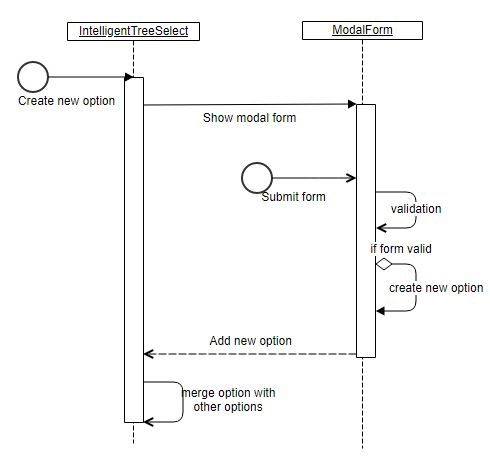
\includegraphics[width=.6\textwidth]{new_option-sequence-diagram}
    \decoRule
    \caption[New option diagram]{Process of creating new option}
    \label{fig:add_new_option}
\end{figure}

%----------------------------------------------------------------------------------------